\documentclass[border=10pt]{standalone}
\usepackage{tikz}
\usepackage{amsmath}
\usetikzlibrary{arrows.meta, calc, positioning, intersections}

\begin{document}
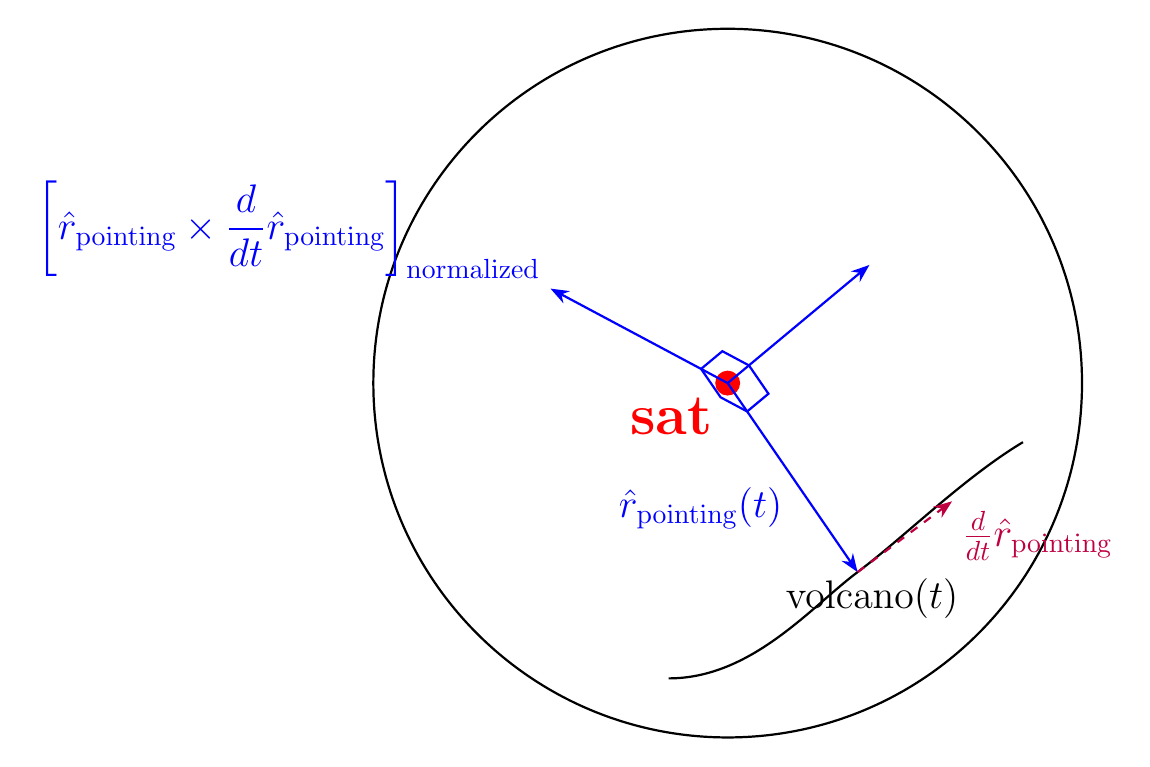
\begin{tikzpicture}[>=Stealth, scale=1.5]

% Define center point (satellite)
\coordinate (sat) at (0,0);

% Draw the big outer circle (representing Earth roughly or orbit plane)
\draw[thick] (sat) circle (3cm);

% Satellite node
\fill[red] (sat) circle (3pt);
\node[below left, text=red, font=\huge\bfseries, xshift=-2pt, yshift=-2pt] at (sat) {sat};

% Draw volcano path EXACTLY through coordinate (1.1, -1.6) so we can place the vector exactly on it
\draw[thick, smooth, name path=volcano_path] 
    (-0.5, -2.5) .. controls (0.2, -2.5) and (0.7, -1.9) .. 
    (1.1, -1.6) .. controls (1.5, -1.3) and (2.0, -0.8) .. 
    (2.5, -0.5) 
    node[pos=0.1, below=0.1cm, text=black, font=\Large] {$\text{volcano}(t)$};

% Pointing vector points EXACTLY to (1.1, -1.6) which is definitely on the black line now
\coordinate (volcano) at (1.1, -1.6);
\draw[->, thick, blue] (sat) -- (volcano) node[midway, below left, align=left, font=\Large] {$\hat{r}_{\text{pointing}}(t)$};

% Tangent vector at (1.1, -1.6). 
% It's tangent to the curve, so it doesn't need a right angle with the pointing vector (unless it's a perfect circle).
\coordinate (deriv) at ($(volcano) + (0.8, 0.6)$); 
\draw[->, thick, purple, dashed] (volcano) -- (deriv) node[below right, font=\Large] {$\frac{d}{dt}\hat{r}_{\text{pointing}}$};

% Draw the other two axes based on the cross product
% Axis 1: The cross product axis (perpendicular to pointing and derivative)
\coordinate (cross_axis) at (-1.5, 0.8);
\draw[->, thick, blue] (sat) -- (cross_axis) node[above left, align=center, font=\Large] {$\displaystyle \left[ \hat{r}_{\text{pointing}} \times \frac{d}{dt}\hat{r}_{\text{pointing}} \right]_{\text{normalized}}$};

% Axis 2: Completing the triad (mutually orthogonal)
\coordinate (triad_axis) at (1.2, 1.0);
\draw[->, thick, blue] (sat) -- (triad_axis);

% Draw right angle symbols properly at the origin for the 3 axes
\coordinate (p_v) at ($(sat)!0.15!(volcano)$);
\coordinate (p_t) at ($(sat)!0.15!(triad_axis)$);
\coordinate (p_c) at ($(sat)!0.15!(cross_axis)$);

\draw[blue, thick] (p_v) -- ($(p_v)+(p_t)-(sat)$) -- (p_t);
\draw[blue, thick] (p_t) -- ($(p_t)+(p_c)-(sat)$) -- (p_c);
\draw[blue, thick] (p_c) -- ($(p_c)+(p_v)-(sat)$) -- (p_v);

\end{tikzpicture}
\end{document}
